\documentclass[a4paper, french, 12pt, titlepage]{report}
\usepackage[latin1, utf8]{inputenc}
\usepackage[T1]{fontenc}
\usepackage{graphicx,  amsmath, amssymb}
\usepackage[margin = 1in]{geometry}
\graphicspath{{./images/}}


\title{Rapport de stage \\ Modélisation numérique d’oscillateurs non-linéaires pour
la récupération d’énergie vibratoire}
\author{LÉGLISE Cloé}

\begin{document}

\maketitle

\section{Introduction}


Ce stage a été réalisé en quatrième année d'école d'ingénieurs, dans le cadre d'un stage obligatoire type "assistant ingénieur" d'une durée minimale de six semaines. 

\section{Contexte du stage}

\subsection{Présentation de l'organisme d'acueil}

L’Université Savoie Mont Blanc (USMB) est un établissement de 15 000 étudiants ouvert sur l’Europe et le monde. Les recherches sont menées par des laboratoires labellisés et reconnus, en partenariats étroits avec de grands organismes (CNRS, CEA, INRA), des organisations internationales (CERN) ou d’autres structures (INES, ”Institut de la Montagne”) à la pointe de l’innovation. Le SYMME (”Systèmes et Matériaux pour la Mécatronique”) est l’un de ces laboratoires. Il a été créé en 2006 pour renforcer la position stratégique de l’université dans le domaine de la mécatronique. Il emploie environ 80 chercheurs, personnel administratif et étudiants. Ses recherches dans le domaine des microsources d’énergie concernent notamment le développement de structures électromécaniques innovantes aux échelles centimétrique et millimétrique, capables de convertir des énergies mécaniques en énergie électrique. Ces travaux recouvrent les aspects mécaniques et électroniques dans une approche multiphysique globale et cohérente. Plus particulièrement, ses activités de recherche portent sur les transducteurs piézoélectriques, électromagnétiques et électrostatiques pour la conversion d’énergie, sur des oscillateurs mécaniques linéaires et non-linéaires pour élargir la bande de fréquence des générateurs, et sur des interfaces électriques pour le conditionnement de l’énergie et le suivi de fréquences. Ses travaux ont fait l’objet de nombreuses communications dans des journaux et des conférences de référence dans le domaine et sont reconnus par la communauté scientifique.\\


Les travaux au laboratoire SYMME suivent deux axes principaux : "Matériaux, Systèmes et Instrumentation Intelligents", et "Qualité Industrielle". Ces deux thèmes sont eux-mêmes divisés en trois thèmes chacuns, respectivement : "Matériaux et nanomatériaux fonctionnels", "Instrumentation pour le médical", et "Valorisation de micro-sources d'énergies ambiantes" ; et "Caraxtérisation et modélisation thermomécanique des matériaux", "Optimisation produit-procédé" et "Optimisation des processus". \\

\begin{figure}
  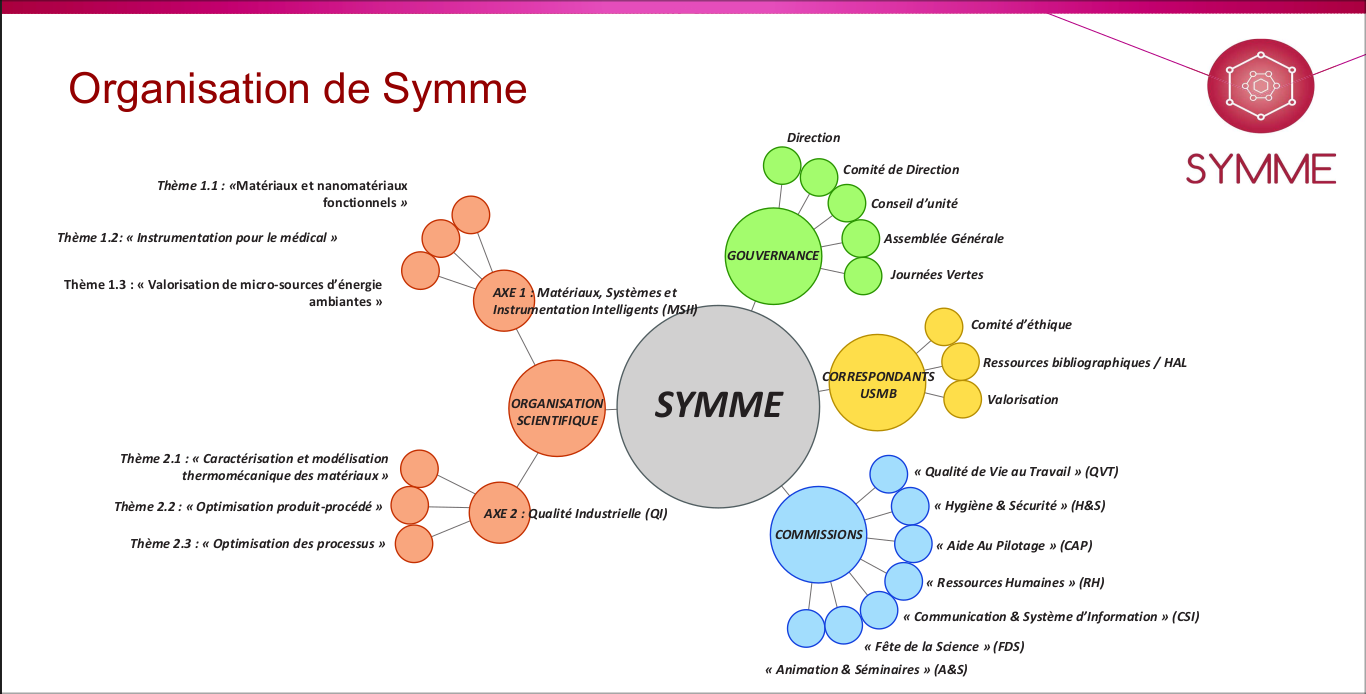
\includegraphics[width=\linewidth]{organigramme.png}
  \caption{Organisation du laboratoire SYMME}
  \label{fig:organigramme}
\end{figure}
La figure 1 montre l'organisation du laboratoire SYMME. 

C'est dans le thème "Matériaux, systèmes et instrumentation intelligents - valorisation de micro-sources d'énergies ambiantes" que s'inscrit ce stage. 

\subsection{Sujet de stage}
Le déploiement de réseaux de capteurs sans fil communicants nécessite l’utilisation de batteries qui ont une durée de vie limitée. Le domaine de la récupération d’énergie vibratoire vise à remplacer, ou du moins complémenter, l’usage de ces batteries au moyen de systèmes innovants de récupération et de stockage d’énergie robustes et fiables. Un récupérateur d’énergie vibratoire est généralement composé d’un oscillateur mécanique, de transducteurs électromécaniques (par exemple des transducteurs piézoélectriques) pour la conversion de l’énergie mécanique des vibrations en énergie électrique et d’un circuit d’extraction électrique. Les premiers travaux dans le domaine utilisaient des récupérateurs linéaires, c’est-à-dire, ceux composés d’un oscillateur linéaire. Cependant, de tels récupérateurs présentent une bande de fréquences étroite et ne sont donc pas adaptés à un environnement présentant un spectre de vibration riche et varié. Une solution prometteuse pour élargir la bande de fréquences est de considérer un oscillateur non-linéaire. Cependant, les comportements des récupérateurs non-linéaires sont plus difficiles à prédire de part l’existence de plusieurs solutions pour une fréquence de vibration donnée. Une analyse approfondie est nécessaire pour une compréhension complète de la dynamique. Dans le cadre du stage, le candidat sera en charge de modéliser un récupérateur non-linéaire développé au sein du laboratoire SYMME et se familiarisera avec les outils numériques déjà mis en place.

L’objectif de ce stage est de développer une interface graphique pour l’analyse d’influence des paramètres du modèle. La dynamique pourra être visualisée sur l’interface. Le projet open-source sera développé en Python ou en Julia. Le stagiaire définira les fonctionnalités de l’application et passera à la phase de développement de l’application. Par exemple, il faudra faire en sorte que l’utilisateur puisse choisir un modèle de récupérateur d’énergie vibratoire, définir le type d’excitation, changer les valeurs numériques des paramètres et choisir les variables qu’il souhaite visualiser. Le stagiaire utilisera un outil de développement logiciel open-source de son choix (Gitlab, GitHub) afin d’assurer une intégration continue et associer une documentation (manuel d’utilisation) à l’application. Durant le stage, le candidat développera ses compétences en développement logiciel et modélisation numérique. Il sera intégré dans une équipe ayant une expertise dans la modélisation, conception et développement de solutions pour la récupération d’énergie, au laboratoire SYMME (Annecy). Selon l’avancement du stage, l’application développée par le stagiaire pourra faire l’objet d’une publication d’un article scientifique.




\section{Résumé des papiers}

L'utilisation de récupérateurs d'énergie permet de récolter de l'énergie vibratoire. Il en existe de plusieurs sortes, par exemple les récupérateurs d'énergie piézoélectriques linéaires, qui peuvent amplifier les vibrations s'ils sont excités à leur fréquence naturelle. Ceci dit, ces récupérateurs d'énergie ne peuvent récupérer une puissance importante qu'au sein d'une bande passante très étroite. Les récupérateurs d'énergie vibratoire non linéaires ont une bande passante bien plus large, bien que la complexité de leurs comportement peuvent les rendre difficiles à analyser. 

Les récupérateurs d'énergie non linéaires multi-stables peuvent présenter plusieurs cycles limites stables, appelés orbites, qui dépendent des conditions initiales. Certaines de ces orbites, appelées orbites hautes, correspondent à un mouvement oscillatoire entre deux positions stables de la masse inertielle. D'autres, appelées orbites basses, correspondent à une situation à la masse inertielle oscille faiblement autour d'une seule position stable. Les orbites hautes sont beaucoup plus intéressantes pour la récupération d'énergie, parce qu'elles représentent une puissance plus importante. Il est donc intéressant de mettre en place des stratégies de saut d'orbites, permettant à l'oscillateur de passer d'une orbite faible à une orbite basse. 

Pour effectuer un saut d'orbite, il faut nécessairement donner de l'énergie à l'oscillateur. Il faut donc trouver une méthode la moins coûteuse en énergie possible pour que la manipulation soit rentable. Pour un oscillateur bistable de Duffing, cinq paramètres jouent un rôle important dans son comportement : la masse M, la raideur k, la valeur des positions stables $x_0$, la longueur L et l'amortissement µ. Notons que le niveau de flambement, donné par $\frac{x_0}{L}$, sera indirectement modifié par la modification d'autres paramètres. Ainsi, en touchant l'un de ces paramètres, on peut augmenter l'énergie potentielle du système et ainsi le faire passer d'une orbite basse à une orbite haute. 


\section{Cahier des charges}

\section{Mise en place}

Durant ce stage, différents outils de travail ont été utilisés. La totalité du code écrit se situe dans un repository Git, dont l'utulisation a permis de travailler en équipe, récupérer d'anciennes versions du code, et l'application finale disponible. La programmation a été réalisée sur l'éditeur de code Visual Studio Code, dont les nombreuses extensions permettent d'utiliser de nombreux langages différents, ainsi que des outils tels que Git de manière rapide et instinctive. Après plusieurs discussions, il a été décidé que la programmation serait faite en utilisant le langage Julia, plus rapide et performant que Python, et avec des librairies simplifiées sur la résolution d'équations différentielles et l'affichage de graphes interactifs. 

\section{Travail effectué}

\section{Ce qu'il reste à faire}

\section{Conclusion}



\section*{Bibliographie}

Saint-Martin, C., Morel, A., Charleux, L., Roux, E., Benhemou, A., \& Badel, A. (2022). Power expectation as a unified metric for the evaluation of vibration energy harvesters. Mechanical Systems and Signal Processing, 181, 109482.

Huguet, T. (2018). Vers une meilleure exploitation des dispositifs de récupération d’énergie vibratoire bistables: Analyse et utilisation de comportements originaux pour améliorer la bande passante (Doctoral dissertation, Université de Lyon).

Liu, W. (2014). Conception d'un dispositif de récupération d'énergie vibratoire large bande (Doctoral dissertation, Grenoble).

	
\end{document}

